
\documentclass[aspectratio=169,11pt]{beamer}

\usetheme{default}
\usecolortheme{default}
\setbeamertemplate{navigation symbols}{}
\setbeamertemplate{footline}[frame number]
\setbeamertemplate{itemize items}[circle]
\setbeamertemplate{enumerate items}[default]

\usepackage[T1]{fontenc}
\usepackage{lmodern}
\usepackage{booktabs}
\usepackage{array}
\usepackage{graphicx}
\usepackage{makecell}
\usepackage{xcolor}
\usepackage{amsmath}
\usepackage{tikz}
\usetikzlibrary{arrows.meta,positioning}

\graphicspath{{../output/figures/}{../output/model/}{../output/empirical/}{../output/exhibits/}}

\definecolor{DVCBlue}{RGB}{25,74,120}
\definecolor{DVCGreen}{RGB}{26,115,85}
\definecolor{DVCGrey}{RGB}{92,96,102}
\definecolor{DVCOrange}{RGB}{170,95,32}

\setbeamercolor{title}{fg=DVCBlue}
\setbeamercolor{frametitle}{fg=DVCBlue}
\setbeamercolor{structure}{fg=DVCBlue}
\setbeamercolor{normal text}{fg=black,bg=white}
\setbeamerfont{title}{series=\bfseries,size=\Large}
\setbeamerfont{frametitle}{series=\bfseries,size=\large}
\setbeamerfont{footnote}{size=\tiny}

\newcommand{\source}[1]{\vfill {\tiny\textcolor{DVCGrey}{#1}}}
\newcommand{\key}[1]{\textcolor{DVCBlue}{\textbf{#1}}}
\newcommand{\good}[1]{\textcolor{DVCGreen}{\textbf{#1}}}
\newcommand{\warn}[1]{\textcolor{DVCOrange}{\textbf{#1}}}

\title{The Making of Vehicle Currencies}
\subtitle{Evidence from DeFi Route-Level Markets}
\author{Jiahua Xu}
\institute{Nanyang presentation draft}
\date{2026}

\begin{document}

\begin{frame}
  \titlepage
\end{frame}

\begin{frame}{Motivation: vehicle currencies are routing infrastructure}
\begin{itemize}
  \item A vehicle currency is not just a large asset or a popular endpoint.
  \item It is an asset that other trades route through when direct exchange is missing, thin, or costly.
  \item Classic foreign-exchange markets make the vehicle role hard to observe directly.
  \item DeFi gives transaction-level routes, liquidity, endpoint tokens, and settlement traces.
\end{itemize}
\vspace{0.4em}
\begin{block}{Research question}
When and why does an asset become the intermediary through which other assets trade?
\end{block}
\end{frame}

\begin{frame}{One-sentence thesis}
\begin{block}{Main claim}
Vehicle currencies are made by route feasibility and liquidity concentration: they protect traders from missing or thin direct markets, persist with vehicle-linked liquidity, rotate under stress, and become more virtual when settlement architecture nets physical token movement.
\end{block}
\vspace{0.8em}
\begin{itemize}
  \item The paper is not a WETH-only story.
  \item WETH, stablecoins, V3, and V4 are empirical test beds for general vehicle-currency mechanisms.
\end{itemize}
\end{frame}

\begin{frame}{Why DeFi is a useful laboratory}
\begin{columns}[T,onlytextwidth]
\begin{column}{0.50\textwidth}
\textbf{What traditional data often hide}
\begin{itemize}
  \item route choice
  \item intermediate asset identity
  \item direct-route availability
  \item execution-cost counterfactuals
  \item settlement implementation
\end{itemize}
\end{column}
\begin{column}{0.46\textwidth}
\textbf{What the DeFi data reveal}
\begin{itemize}
  \item reconstructed multi-hop routes
  \item exact source, destination, vehicle token
  \item pool liquidity and LP allocation
  \item route-cost quotes and no-direct cases
  \item receipt-level transfer incidence
\end{itemize}
\end{column}
\end{columns}
\end{frame}

\begin{frame}{Measurement: separate endpoint demand from bridge use}
\begin{block}{Main vehicle-use proxy}
\[
\text{BridgeShare}_{k,t}
= \frac{\text{USD volume of indirect routes where }k\text{ is intermediate}}
{\text{USD volume of all indirect routes}}
\]
\end{block}
\begin{itemize}
  \item Main object is conditional on indirect routing.
  \item All-route bridge share reports economic scope.
  \item Endpoint share is a control/diagnostic, not the vehicle proxy.
\end{itemize}
\source{Evidence packet Table 1 / Table 2.}
\end{frame}

\begin{frame}{Route objects}
\centering
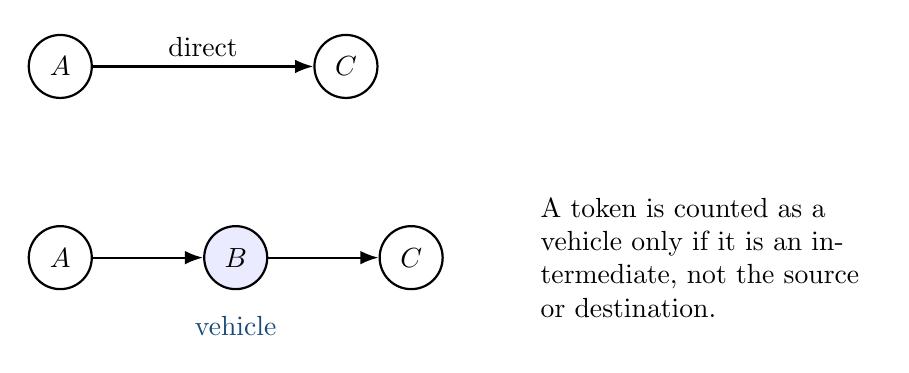
\begin{tikzpicture}[node distance=1.7cm,>=Latex,thick]
\node[draw,circle,minimum size=0.8cm] (A) {$A$};
\node[draw,circle,minimum size=0.8cm,right=2.8cm of A] (C) {$C$};
\draw[->] (A) -- node[above]{direct} (C);

\node[draw,circle,minimum size=0.8cm,below=1.6cm of A] (A2) {$A$};
\node[draw,circle,minimum size=0.8cm,right=1.4cm of A2,fill=blue!8] (B) {$B$};
\node[draw,circle,minimum size=0.8cm,right=1.4cm of B] (C2) {$C$};
\draw[->] (A2) -- (B);
\draw[->] (B) -- (C2);
\node[below=0.2cm of B,text=DVCBlue] {vehicle};

\node[align=left,right=1.1cm of C2,text width=4.2cm] {A token is counted as a vehicle only if it is an intermediate, not the source or destination.};
\end{tikzpicture}
\end{frame}

\begin{frame}{Empirical spine}
\begin{enumerate}
  \item \key{Formation:} direct-market incompleteness and thin-direct protection.\newline
  Evidence: route availability, depth, and cost advantage predict vehicle use.
  \item \key{Liquidity:} liquidity and route use persist together.\newline
  Evidence: LP concentration predicts BridgeShare; lagged BridgeShare predicts future LP.
  \item \key{Stress:} risky incumbent loses share on impact.\newline
  Evidence: WETH-minus-stable share falls on stress days.
  \item \key{Architecture:} direct-market deepening reduces vehicle dependence.\newline
  Evidence: post-V3 no-direct/WETH cases fall.
  \item \key{Settlement:} netting separates route use from physical movement.\newline
  Evidence: V4 lowers intermediary-token transfer incidence.
\end{enumerate}
\end{frame}

\begin{frame}{Proposition 1: direct-market incompleteness}
\begin{block}{Statement}
For an endpoint pair, a candidate vehicle expands the feasible execution set when the direct route is unavailable or thin. Conditional on both routes being feasible, the vehicle route improves execution only when its route cost is below the direct-route cost.
\end{block}
\vspace{0.6em}
\textbf{Empirical margins}
\begin{itemize}
  \item no-direct, vehicle-available cases
  \item thin direct route, vehicle route available
  \item common-support cost advantage
  \item vehicle-route depth
\end{itemize}
\end{frame}

\begin{frame}{Result 1: formation loads on route opportunity}
\scriptsize
\begin{tabular}{lccc}
\toprule
 & Actual vehicle share & Vehicle share $t+7$ & Vehicle share $t+30$ \\
\midrule
Route-cost advantage, per 100 bp & $0.1462^{***}$ & $0.0001^{***}$ & $0.0002^{***}$ \\
 & $(p<0.001)$ & $(p=0.002)$ & $(p<0.001)$ \\
Vehicle-route availability & $19.1385^{***}$ & $0.0940^{***}$ & $0.1254^{***}$ \\
 & $(p<0.001)$ & $(p<0.001)$ & $(p<0.001)$ \\
Vehicle-route depth & $28.8502^{***}$ & & \\
 & $(p<0.001)$ & & \\
LP concentration & & $0.1117^{***}$ & \\
 & & $(p<0.001)$ & \\
Lagged vehicle share & & & $0.3630^{***}$ \\
 & & & $(p<0.001)$ \\
\midrule
FE & pair $\times$ date & token, date & token, date \\
Observations & 189,143 & 9,380 & 9,265 \\
\bottomrule
\end{tabular}
\source{Evidence packet Table 4.}
\end{frame}

\begin{frame}{Result 1 interpretation}
\begin{itemize}
  \item The vehicle role is not simply ``the cheapest route everywhere.''
  \item The strongest interpretation is \key{availability and thin-direct protection}.
  \item Common-support cost advantage is one mechanism, but not the whole vehicle value.
  \item This framing is important for not making a false universal-cheaper-route claim.
\end{itemize}
\end{frame}

\begin{frame}{Proposition 2: liquidity-route persistence}
\begin{block}{Statement}
Vehicle-linked liquidity and vehicle use are jointly persistent: liquidity around a candidate vehicle predicts future vehicle use, and current vehicle use predicts future vehicle-linked liquidity.
\end{block}
\vspace{0.6em}
\begin{itemize}
  \item This is a reduced-form persistence claim.
  \item It is not yet an exogenous LP-shock causal design.
\end{itemize}
\end{frame}

\begin{frame}{Result 2: liquidity and route use predict each other}
\scriptsize
\begin{tabular}{lccc}
\toprule
 & Vehicle share $t+7$ & LP concentration $t+7$ & Log LP liquidity $t+7$ \\
\midrule
LP concentration & $0.1117^{***}$ & & \\
 & $(p<0.001)$ & & \\
Lagged vehicle share & & $0.0419^{***}$ & $1.1713^{***}$ \\
 & & $(p<0.001)$ & $(p<0.001)$ \\
\midrule
FE & token, date & token, date & token, date \\
SE clustering & date & date & date \\
Observations & 9,380 & 9,380 & 9,380 \\
\bottomrule
\end{tabular}
\vspace{0.8em}
\begin{itemize}
  \item Liquidity concentration predicts future vehicle use.
  \item Vehicle use predicts future vehicle-linked liquidity.
\end{itemize}
\source{Evidence packet Table 5.}
\end{frame}

\begin{frame}{Figure: vehicle shares and liquidity}
\centering
\includegraphics[width=0.86\textwidth,height=0.72\textheight,keepaspectratio]{figure_04_lp_concentration_timeseries.pdf}
\source{Generated exhibit: LP concentration time series.}
\end{frame}

\begin{frame}{Proposition 3: impact stress rotation}
\begin{block}{Statement}
A risk or credibility shock to an incumbent vehicle reduces its route-intermediation share on impact relative to safer substitutes, conditional on common route opportunities.
\end{block}
\vspace{0.5em}
\begin{itemize}
  \item Model is interval-neutral: it predicts an impact response.
  \item Empirically strongest at the same-day event window.
  \item Hourly/weekly results are useful duration/noise diagnostics, not the headline.
\end{itemize}
\end{frame}

\begin{frame}{Result 3: stress rotates away from WETH}
\scriptsize
\begin{tabular}{lccccc}
\toprule
 & WETH share & Stable share & WETH-stable gap & Direct share & Indirect volume \\
\midrule
Stress event day & $-1.48^{**}$ pp & $1.48^{**}$ pp & $-2.96^{**}$ pp & $-0.25$ pp & $0.51^{***}$ log pts \\
 & $(p=0.018)$ & $(p=0.018)$ & $(p=0.018)$ & $(p=0.679)$ & $(p=0.005)$ \\
\bottomrule
\end{tabular}
\vspace{0.8em}
\begin{itemize}
  \item Same-day common-support rotation is the cleanest stress result.
  \item Threshold and non-overlap checks remain negative and statistically significant.
\end{itemize}
\source{Evidence packet Table 6.}
\end{frame}

\begin{frame}{Figure: common-support stress rotation}
\centering
\includegraphics[width=0.88\textwidth,height=0.72\textheight,keepaspectratio]{figure_05_stress_common_support.pdf}
\source{Generated exhibit: stress common-support vehicle rotation.}
\end{frame}

\begin{frame}{Proposition 4a: direct-market-deepening architecture}
\begin{block}{Statement}
An architecture that increases direct pairwise depth reduces reliance on vehicle routes that exist only because the direct route is absent or thin.
\end{block}
\vspace{0.6em}
\begin{itemize}
  \item Empirical test bed: concentrated-liquidity launch.
  \item Defensible claim: no-direct/WETH-available cases fall.
  \item Do not claim every V3 outcome has clean causal timing.
\end{itemize}
\end{frame}

\begin{frame}{Result 4a: V3 reduces no-direct dependence}
\scriptsize
\begin{tabular}{lcccc}
\toprule
 & No-direct WETH & Q1 direct & Q1 no-direct & Q2 no-direct \\
\midrule
Post V3 & $-25.81^{***}$ & $56.42^{***}$ & $-33.03^{***}$ & $-47.51^{***}$ \\
 & $(p<0.001)$ & $(p<0.001)$ & $(p=0.007)$ & $(p<0.001)$ \\
\midrule
FE & pair & pair & pair & pair \\
SE clustering & pair & pair & pair & pair \\
\bottomrule
\end{tabular}
\vspace{0.8em}
\begin{itemize}
  \item Strongest message: architecture can reduce vehicle dependence by expanding direct-route opportunity.
\end{itemize}
\source{Evidence packet Table 7.}
\end{frame}

\begin{frame}{Proposition 4b: settlement netting}
\begin{block}{Statement}
Settlement netting can preserve the route-pricing role of a vehicle while reducing physical transfers of the intermediary token.
\end{block}
\vspace{0.6em}
\begin{itemize}
  \item Empirical test bed: matched V3 and V4 route units.
  \item Route vehicle use and physical settlement movement become separable objects.
\end{itemize}
\end{frame}

\begin{frame}{Result 4b: V4 virtualizes part of the vehicle role}
\scriptsize
\begin{tabular}{lcccc}
\toprule
 & All sizes & Small & Medium & Large \\
\midrule
V4 - V3 transfer incidence & $-18.6^{***}$ pp & $-39.4^{***}$ pp & $-12.3^{***}$ pp & $-3.2^{*}$ pp \\
 & $(p<0.001)$ & $(p<0.001)$ & $(p=0.002)$ & $(p=0.083)$ \\
V3 transfer incidence & 100.0\% & 100.0\% & 100.0\% & 100.0\% \\
V4 transfer incidence & 81.4\% & 60.6\% & 87.7\% & 96.8\% \\
\bottomrule
\end{tabular}
\vspace{0.8em}
\begin{itemize}
  \item V4 does not eliminate vehicle currencies.
  \item It makes part of the vehicle role virtual: the token can remain the route intermediary without moving physically in every route unit.
\end{itemize}
\source{Evidence packet Table 8.}
\end{frame}

\begin{frame}{Figure: settlement-transfer incidence}
\centering
\includegraphics[width=0.88\textwidth,height=0.72\textheight,keepaspectratio]{figure_06_v4_settlement_transfer_incidence.pdf}
\source{Generated exhibit: V4 settlement transfer incidence.}
\end{frame}

\begin{frame}{Additional mechanism: common vehicle-linked liquidity}
\tiny
\begin{tabular}{lccccc}
\toprule
 & Full & Stress & High veh. & Low veh. & Excl. top \\
\midrule
Market factor & $0.7063^{***}$ & $0.6987^{***}$ & $0.6572^{***}$ & $0.5276^{***}$ & $0.7062^{***}$ \\
 & $(p<0.001)$ & $(p<0.001)$ & $(p<0.001)$ & $(p<0.001)$ & $(p<0.001)$ \\
Vehicle factor & $0.1626^{***}$ & $0.1586^{***}$ & $0.2174^{***}$ & $-0.0921$ & $0.1670^{***}$ \\
 & $(p<0.001)$ & $(p<0.001)$ & $(p<0.001)$ & $(p=0.307)$ & $(p<0.001)$ \\
Vehicle factor $\times$ stress & & $0.1064^{**}$ & & & \\
 & & $(p=0.030)$ & & & \\
\bottomrule
\end{tabular}
\vspace{0.8em}
\begin{itemize}
  \item Same-vehicle pools share a liquidity component beyond market-wide liquidity.
  \item This can be a main slide or a backup, depending on time.
\end{itemize}
\source{Evidence packet Table 9.}
\end{frame}

\begin{frame}{What the evidence supports}
\begin{enumerate}
  \item \key{Formation:} route opportunity and depth predict vehicle use.
  \item \key{Persistence:} vehicle use and vehicle-linked liquidity are persistent together.
  \item \key{Rotation:} stress moves flow away from risky incumbent vehicle use toward stable substitutes on impact.
  \item \key{Architecture:} market design changes direct-route feasibility.
  \item \key{Settlement:} netting separates route intermediation from physical token movement.
\end{enumerate}
\end{frame}

\begin{frame}{What the evidence does not claim}
\begin{itemize}
  \item Not: WETH is always the cheapest route.
  \item Not: liquidity feedback is causally identified from an exogenous LP shock.
  \item Not: stress rotation is a permanent regime shift in every window.
  \item Not: V4 removes vehicle currencies.
  \item Not: Curve/Fluid are exact-quoted in the main route-cost panel.
\end{itemize}
\vspace{0.6em}
\begin{block}{Paper discipline}
The strongest contribution comes from bounded claims that match the actual empirical objects.
\end{block}
\end{frame}

\begin{frame}{Contribution}
\begin{itemize}
  \item \textbf{Vehicle-currency literature:} measures vehicle use directly as route intermediation.
  \item \textbf{Liquidity/intermediation literature:} shows vehicle status is tied to liquidity concentration and route opportunity.
  \item \textbf{Market design:} shows architecture changes vehicle reliance and settlement implementation.
  \item \textbf{DeFi evidence:} turns transparent route-level ledgers into a laboratory for classic monetary intermediation questions.
\end{itemize}
\end{frame}

\begin{frame}{Next decisions for the Nanyang talk}
\begin{itemize}
  \item How technical should the model section be for this audience?
  \item Should common liquidity be main-deck or backup?
  \item How much DeFi institutional detail is needed before the results?
  \item Which result should be the punchline: liquidity formation, stress rotation, or V4 virtualization?
\end{itemize}
\vspace{0.6em}
\begin{block}{My recommendation}
Lead with measurement and formation, use stress and V4 as sharp payoffs, keep common liquidity as backup unless the audience is strongly market-microstructure focused.
\end{block}
\end{frame}

\begin{frame}{Conclusion}
\begin{block}{Takeaway}
Vehicle currencies are not just dominant assets. They are route-level liquidity institutions whose role depends on direct-market incompleteness, liquidity concentration, stress-state substitution, and settlement architecture.
\end{block}
\end{frame}

\end{document}
